\documentclass[29pt,a4paper]{moderncv}

% moderncv themes
%\moderncvtheme[blue]{casual}                 % optional argument are 'blue' (default), 'orange', 'red', 'green', 'grey' and 'roman' (for roman fonts, instead of sans serif fonts)
\moderncvtheme[green]{banking}                % idem

\usepackage[T1]{fontenc}
% character encoding
\usepackage[utf8x]{inputenc}               	% replace by the encoding you are using
\usepackage[italian]{babel}
\usepackage{color}

% adjust the page margins
\usepackage[scale=0.8]{geometry}
\recomputelengths                          	% required when changes are made to page layout lengths

\fancyfoot{} % clear all footer fields
\fancyfoot[L,RO]{\thepage}           		% page number in "outer" position of footer line
\fancyfoot[R,LO]{\footnotesize} 			% other info in 


\begin{document}


\section{\textbf{Table of Contents:}}
\begin{tabbing}
\\\textbf{Subject}: ~~~~~\= ~~~~~~~~~~~~~~~~~~~~~~~~~~~~~~~~~~~~~~~~~~~~~~~~~~~~~~~~~~~~~~~~~~~~~~~~~~~~~~~~~~~~~~~\= \textbf{Page}:
\\\newline
1. About TeXchat \> \> 2\\
2. TeXchat vs. SMS \> \> 2\\
3. User Guide: Getting started\> \> 2\\
4. Configuration \> \> 3 \\
5. User Login	\> \> 4			\\
6. User Logout \> \> 5 	\\
7. Remember Me \> \> 5\\
8. User Registration \> \> 6 	\\
9. Adding a Contact\> \> 7 	\\
10. Send Message \> \> 8\\
11. Create Expression \> \> 10\\
12. Delete Chat History \> \> 11 	\\
13. Closing the Application \> \> 12 	\\
\end{tabbing}

\newpage
	%\maketitle
	%\vspace{-10mm}
	%Section
	\section*{\textbf{1. About TeXchat}}
	\vspace{4mm}
			\\TeXchat is an open source messaging application that is developed for the Android platform and works in a similar fashion to normal SMS services.  It works through a Jabber server which connects users and allows communication.  It was originally developed to support users that need to collaborate and communicate in a mathematical or scientific environment, therefore allowing them to effectively construct and send mathematical expressions in line with plain text messages. It is supported by most android platforms from version 2.2 through 4.3.\\
		\vspace{5mm}
		
\section*{\textbf{2. TeXchat vs. SMS}}
	\vspace{4mm}
		 \\TeXchat works in a similar fashion to normal SMS services. SMS is an older and limited messaging system that has limited capabilities, specifically it supports mostly plain text messages and at a relatively high cost. \\ 
		 
		 The TeXchat application allows this basic plain text messaging functionality, and includes the ability for users to construct, edit and view mathematical expressions and then add them as images inline to the rest of the plain text message body.  This feature makes TeXchat unique and supports anyone in an educational, mathematical or scientific environment who may have a need to communicate effectively using such mathematical expressions. \\  
		 
		 The TeXchat messaging service is freely available online, and uses an open and free Jabber server.  Therefore using the TeXchat service has no additional cost to the user except the bandwidth used to exchange data, which is another advantage of making use of this messenger service as opposed to using the older and conventional SMS service.   \\
	\vspace{5mm}
		
	\section*{3. User Guide: Getting Started}
	\vspace{4mm}
	\\Once you have the application correctly installed and configured to an available online Jabber server, you can click on the TeXchat icon and this will open the application Login Page.  
	
	\\This is the TeXchat icon that will be displayed on your device menu, once you have the application installed.
	
	\\For more information on how to configure your device with an available online Jabber server see the Configuration section below.
	
	\vspace{5mm}

\newpage
	\section*{4. Configuration}
	\\To access the Configuration/Settings page, open the application, after you have installed it on your device,press the back button on your device. This will take you to a blank page. Press the menu button, then click on Settings. This will open the settings page where you can configure your details. \\
	\\\textbf{Host name} will contain the name of your jabber host, for example, jabber.iitsp.com. 
	\\\textbf{Server name} will have the name of your jabber host, for example, jabber-0-1.virt.iitsp.com\\
	 Click on Host name and Server name to change the current settings.
	
	\noindent\begin{figure*}
					\centering
					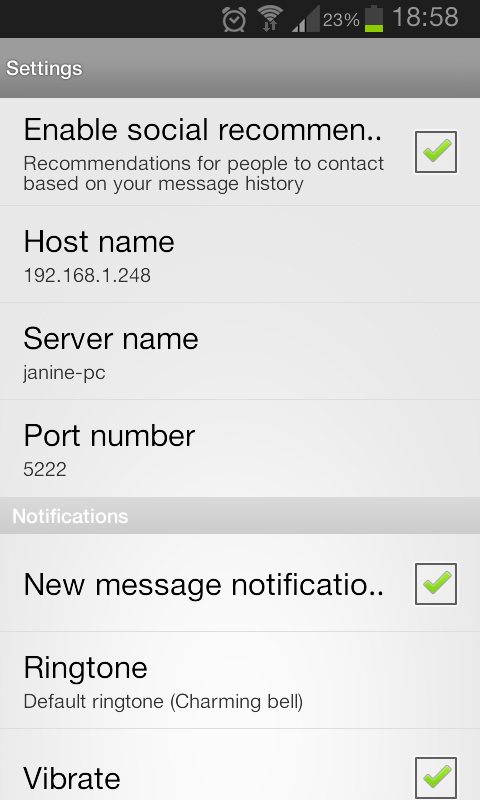
\includegraphics[width=2.5in, height=4.0in]{./Screenshot_2013-10-23-18-58-53.png} \\
					\centering \caption{[Figure 1] Configuration page}
					\end{figure*}\\ 
\newpage
		
\newpage
		\section*{5. User Login}
		\vspace{4mm}
		\\The login page is displayed once the application is opened.  
		
		\\A user that is already registered to use the TeXchat service may simply enter his/her selected username and password in the corresponding fields on the login page, then click on the Login button displayed below.  You should then see the login dialog appear, that is displayed while the application attempts to log in to the Jabber server.  Once this operation is completed, you will see your contact list displayed.\\ 
		
		If you are a first time user, you will be greeted with a message after successfully logging in: \textit{"You currently do not have any contacts.  Select the menu option to add a contact."} \\
		\\For information on how to add a contact, see the Adding a Contact sub section below.\\
		
		\\If you already have contacts added to your account, you will see a contact list displayed, which will also provide information regarding the availability of any particular contact.  If a contact is currently offline, the text offline is displayed below the contact’s name, and similarly for contacts that are currently available.\\
		
		\noindent\begin{figure*}
							\centering
							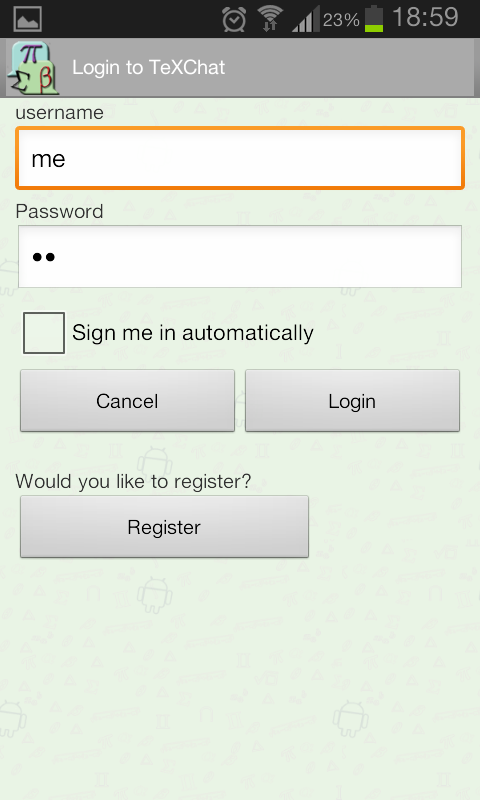
\includegraphics[width=2.5in, height=4.0in]{./Screenshot_2013-10-23-18-59-04.png} \\
							\centering \caption{[Figure 2] Login page}
							\end{figure*}\\ 
		\vspace{5mm}

\newpage
		\section*{7. User Logout}
		\vspace{5mm}
		\\If you are currently logged in to the TeXchat application and wish to log out of your account, you can select the menu key option on your device, and select the Logout option.  You should see the logout dialog appear, that is displayed while the application attempts to log you out from the Jabber server.  Once the operation has completed, you are successfully logged out of your account.\\
		\vspace{4mm}
				
		\section*{8. Remember Me}
		\vspace{5mm}
		\\If you open the application, and see the login page appear after successfully signing in, you will see the Remember Me option presented to you on the login page.  When you select the check box, the application will save your login details, and automatically log you in to your account. \\ 
		
		\\This automatic sign in feature is provided for cases in which the application is abruptly closed, or the application crashed for any reason or simply for user convenience.  The Remember Me information is securely stored locally on your android device and will remain up until you explicitly select the Logout option from your device’s menu. Only once you have explicitly logged out, will the remember me feature be disabled.  \\
		
		\noindent\begin{figure*}
									\centering
									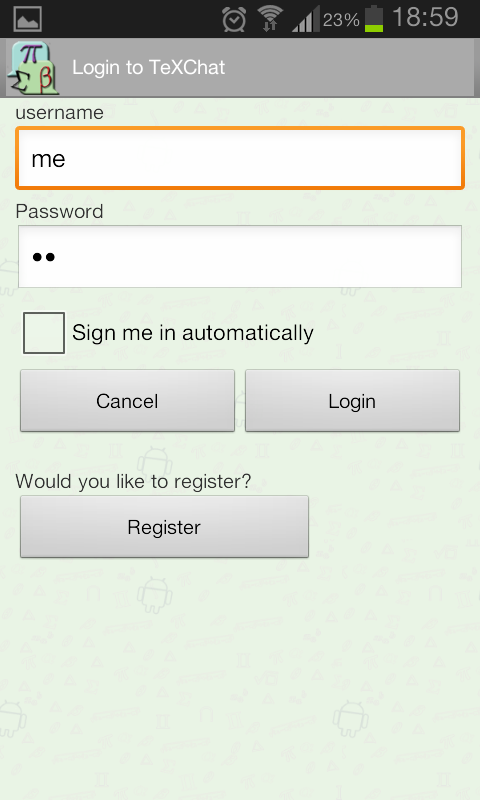
\includegraphics[width=2.5in, height=4.0in]{./Screenshot_2013-10-23-18-59-04.png} \\
									\centering \caption{[Figure 3] Remember me option}
									\end{figure*}\\ 
		\vspace{4mm}
		
\newpage

		\section*{9. User Registration}
		\vspace{5mm}
		\\If you are a first time user, and would like to use the TeXchat messenger application, you will have to register as a user on the server first.  To do this, you can install the application, and click on the icon to start the application.  The first page you will see once the application is running is the login page.  On the login page, you will see the Register button, which you can click on, and this will open the registration form.  
		
		\noindent\begin{figure*}
		\centering
		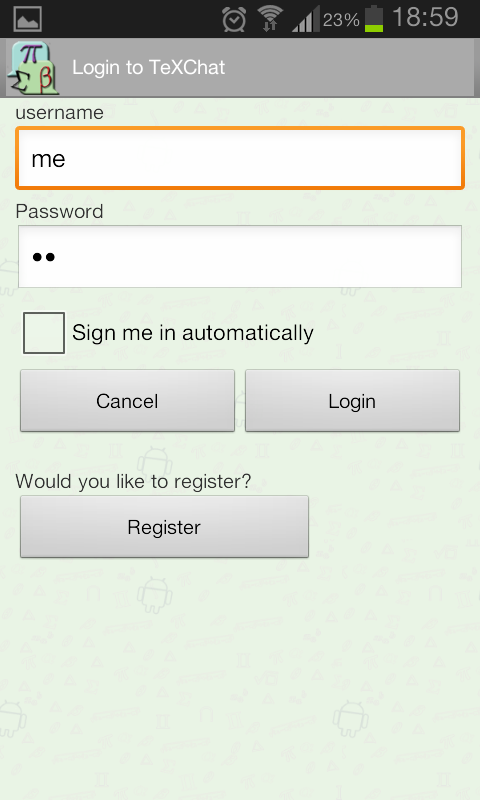
\includegraphics[width=2.5in, height=4.0in]{./Screenshot_2013-10-23-18-59-04.png} \\
		\centering \caption{[Figure 4] Login page with Register button}
		\end{figure*}\\
		
		\\The registration form has various required fields for you to fill in, including your TeXchat username, your display name and password.  Once you have completed the form, you can click on the Register button.  If the message appears, \textit{"Your registration was successful"} you are a valid registered user and you can log in using your chosen username and password combination on the login page. \\
		
		\\If the message appears, \textit{"Registration failed"} you have not been successfully registered and may need to check your connection with the server, and your configuration settings.  If your device is not properly configured to use an available online Jabber server, you will not be able to register.\\
		
		\\Also ensure that all the input text fields are correctly completed, and that both the password fields match before you click on the Register button.  If you decide that you no longer wish to register to the TeXchat application, you can simply click on the Cancel button at the bottom left of the registration form.\\
		
		\noindent\begin{figure*}
		\centering
		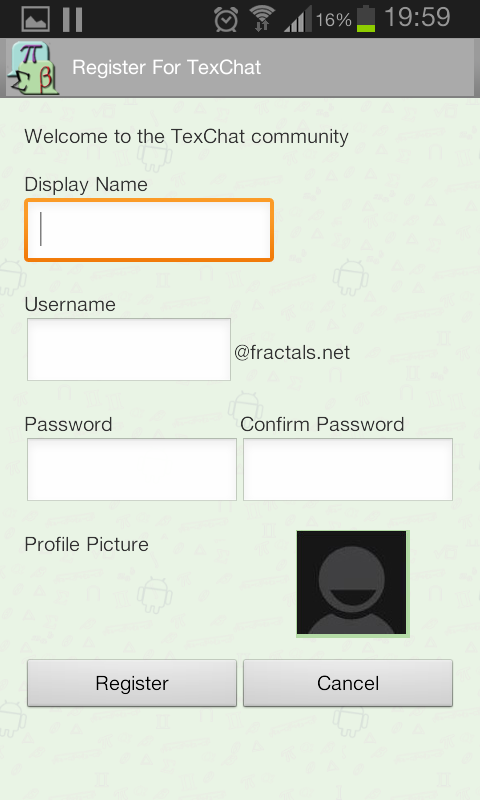
\includegraphics[width=2.5in, height=4.0in]{./Screenshot_2013-10-23-19-59-51.png} \\
		\centering \caption{[Figure 5] Register page}
		\end{figure*}\\
		
		\\[Note: The option to register a user profile picture is not available in V1.0 of the TeXchat application.]
		\vspace{4mm}
		
		\section*{9. Adding a Contact}
				\vspace{5mm}
				To add a contact, whilst you are in your contact list page, press the menu key on your device. Select add contact. The following page will be displayed:\\
				\noindent\begin{figure*}
				\centering
				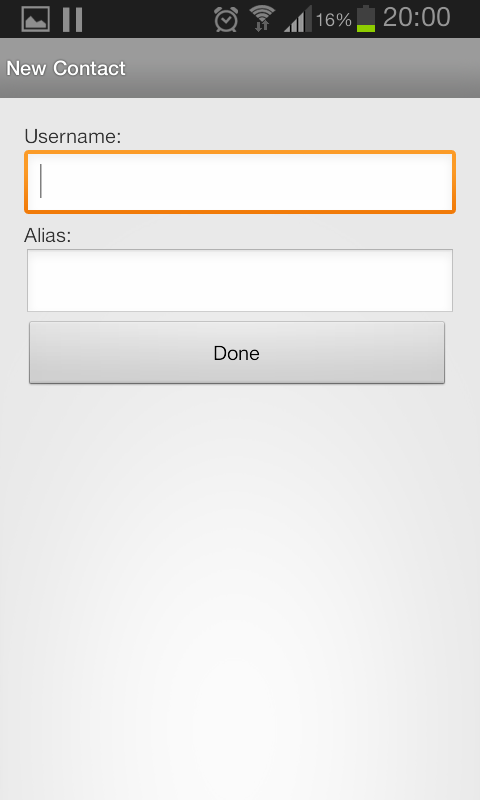
\includegraphics[width=2.5in, height=4.0in]{./Screenshot_2013-10-23-20-00-25.png} \\
				\centering \caption{[Figure 6] Add contact page}
				\end{figure*}\\
				
				\vspace{4mm}
				
		\section*{10. Send Message}
				\vspace{5mm}
				\\From your contact list page, you can open an active chat with any one contact by simply clicking on the contact’s name.  This will open a page that displays all the previous messages between you and that contact if any.  This page will also display the name of the contact you selected in the title bar, so you can easily see the name of the contact with which you are currently communicating.\\
				
				\noindent\begin{figure*}
								\centering
								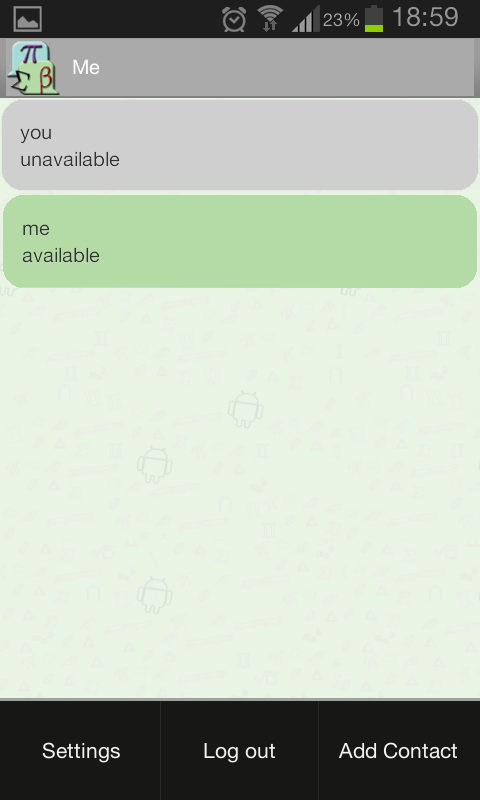
\includegraphics[width=2.5in, height=4.0in]{./Screenshot_2013-10-23-18-59-23.png} \\
								\centering \caption{[Figure 7] Contact List}
								\end{figure*}\\
				
				\\[Note: Green contacts, are online contacts, grey contacts are offline contacts.]\\
				
				\\If you have a message history with the contact you have selected, you should see the relevant messages displayed in similar fashion as below.\\
				
				\noindent\begin{figure*}
				\centering
				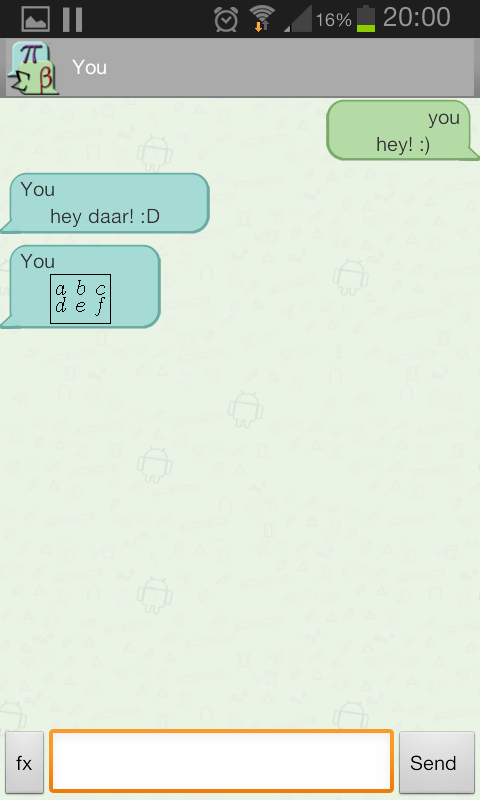
\includegraphics[width=2.5in, height=4.0in]{./Screenshot_2013-10-23-20-00-45.png} \\
				\centering \caption{[Figure 8] Chat History}
				\end{figure*}\\
				
				\\In the case that there is no previous messages recorded between you and the contact you have selected, you will see a messaging page open, simply containing this information displayed as text.\\
				
			\\	\textbf{To send a plain text message} you can type the body of your message in the editable input text field and click on the Send button that is located to the right of the input text field. This will effectively send the plain text you have entered to the contact you have selected.\\  
				
				\\Once you have clicked Send the page will be updated and include the message just sent in the view listing all messages between you and the selected contact.\\
				
			\\	\textbf{To send a message containing expressions} you can click on the fx button displayed to the left of the input text field.  This will open a new page that has another input text field in which you can enter the Latex based expression syntax. Once you are done editing and viewing the expression on this page, you can click on the Add button to the right of the input text field, and this will take you back to the messaging page, with the expression added in the body of text message you are writing. For more information on how to create and edit expressions, see the Create Expression section below.\\
				\vspace{4mm}
				
				\section*{11. Create Expression}
				\vspace{5mm}
				To create an expression, click on the fx button. As seen in the chat page.\\
				\noindent\begin{figure*}
				\centering
				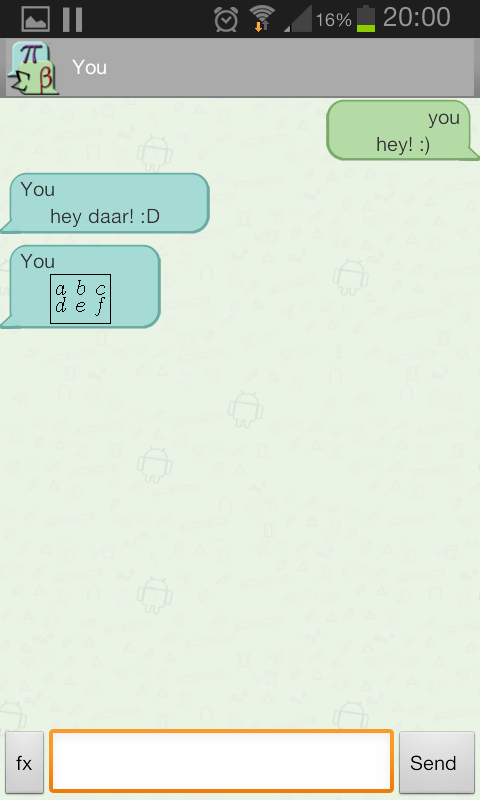
\includegraphics[width=2.5in, height=4.0in]{./Screenshot_2013-10-23-20-00-45.png} \\
				\centering \caption{[Figure 8] Chat page}
				\end{figure*}\\
				
				\\This will open the expression page, in this page you can type the latex math expression in the input box.
				There are various buttons on this page, view, add and \^. \\
				\\The view button gives you a preview of the expression you have designed so far.\\
\\				The add button add the expression  inline with your message you were typing in the chat page.\\
				The \^ button, gives a few predefined expressions and function that you can use. By clicking on one of the images, the expression in the image will be added to the input box above it where you are currently typing you expression.\\
				
				\noindent\begin{figure*}
								\centering
								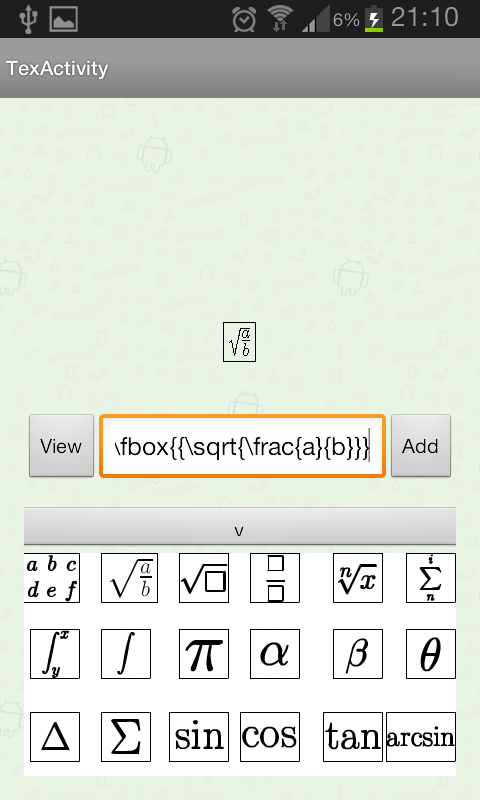
\includegraphics[width=2.5in, height=4.0in]{./Screenshot_2013-10-23-21-10-16.png} \\
								\centering \caption{[Figure 9] Math Expression page}
								\end{figure*}\\
					
				\vspace{4mm}
		
		\section*{12. Delete Chat History}
			\vspace{5mm}
			\\To delete all the messages between you and a contact, you can select the relevant contact from your contact list, and open the chat window.  From this chat window you can open the list of menu options on you device.  Once you select the menu option Delete Chat, all the messages, including chat histories will be permanently deleted from the application and your device and will not be recoverable at any later stage. \\
			\noindent\begin{figure*}
							\centering
							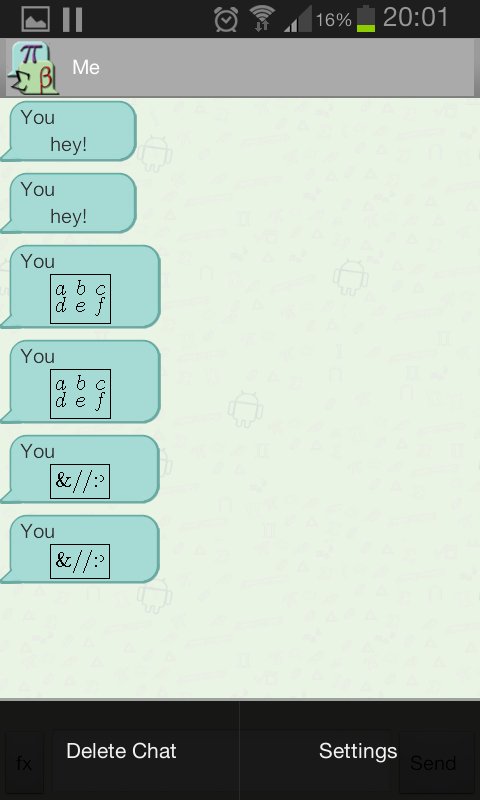
\includegraphics[width=2.5in, height=4.0in]{./Screenshot_2013-10-23-20-01-05.png} \\
							\centering \caption{[Figure 10] Delete Chat}
							\end{figure*}\\
							
			\vspace{5mm}
			
			\section*{113. Closing the Application}
				\vspace{5mm}
				\\To close the application you can click on your device's home button or the back button and this will minimize the application, it will basically still run in the background. You don't have to log in again you can just open the application.
			
				\vspace{4mm}
		
\end{document}